\section{Introduction}\label{sec:introduction}

Spatial and immersive audio techniques have been the beneficiaries of
significant research interest over the past few decades.
Recent developments in virtual and augmented reality technologies and
\textit{object-based} audio have led to an acceleration in interest in the
creation of virtual sound fields via approaches such as Wave Field Synthesis
(WFS) and Higher Order Ambisonics (HOA)~\citep{berkhout_acoustic_1993,
    ahrens_theory_2008,daniel_further_2003,frank_producing_2015}.
These techniques call for the deployment of large numbers of loudspeakers, and
centralised, \textit{in situ} installations of dedicated hardware and software.
The costs associated with such installations have seen them largely restricted
to the preserve of concert venues, cinemas, and institutions with the means to
purchase and operate large-scale systems of this sort.

Advancements in embedded computing mean that there now exist an assortment of
small, low-cost devices with support for audio digital signal processing (DSP).
These devices are open source, relatively easy to program, and may provide
support for communication over ubiquitous computer networking equipment and
protocols.
A network of such devices could be used to \textit{distribute} the problem of
audio spatialisation, potentially lowering the barrier to entry to what is
otherwise a comparatively exclusive branch of audio research.

In this article \textemdash{} which is adapted from a master's thesis written by
the corresponding author, and builds on previous work on a microcontroller-based
networked audio client~\citep{rushton_microcontroller-based_2023} \textemdash{}
we describe the development of a distributed system for spatial and immersive
audio.

\subsection{Networked Audio}\label{subsec:networked-audio}

The transmission of audio data has been a topic of research interest since the
earliest days of computer networking as it is recognised today, i.e.\ over
packet-switched networks, whereby data to be transmitted is grouped into
packets, each consisting of a header and a payload.
Voice transmission over ARPANET was being conducted as early as
1974~\citep{schulzrinne_voice_1992} and the first standard for voice
communication over packet-switched networks \textemdash{} the Network Voice
Protocol (NVP) \textemdash{} was released in
1977~\citep{cohen_specifications_1977}.

With its references to `calling' and `ringing', it is clear that the NVP
standard was intended for digital telephony.
Indeed, research on networked audio was primarily concerned with telephony well
into the 1990s, focusing on real-time voice communication over wide area
networks (WAN) with efforts centring on \textit{quality of service} (QoS),
particularly with regard to the perennial issues of latency, packet loss, and
network jitter \textemdash{} inconsistencies in the rate of packet
transmission~\citep{hardman_reliable_1995,hardman_successful_1998}.
Work at this time dealt with streams of compressed audio data, and speech
coding algorithms to overcome the deleterious effects of dropped packets over
unreliable network paths and low-bandwidth connections.

Whereas the priority for digital telephony, and later voice over IP (VoIP)
systems, is intelligibility, for musical purposes fidelity, and the use of
uncompressed audio signals, is of greater concern.
With the increasing availability of high-speed internet connections in the late
1990s came research into transmitting uncompressed audio data over the
internet~\citep{chafe_simplified_2000,xu_real-time_2000}.
Work of this sort was spearheaded by the \textit{SoundWIRE} project, developed
by researchers at McGill University and Stanford University, and took the form
of a wide variety of experiments with high quality audio over both WAN and local
area networks (LAN).
These experiments included LAN-based real-time musical
performances~\citep{chafe_simplified_2000}, concert streaming over
WAN~\citep{xu_real-time_2000,chafe_simplified_2000}, and sonification of QoS via
a distributed digital waveguide dubbed the
\textit{Network Harp}~\citep{chafe_simplified_2000,chafe_physical_2002}

\subsubsection{Protocols and Systems}\label{subsubsec:protocols-systems}

VoIP research in the 1990s focused on matters such as audio codecs and data
compression~\citep{turletti_inria_1995,hardman_successful_1998}, seeking a
compromise with the \textit{best-effort} nature of internet service.
The SoundWIRE project, in search of high audio quality, turned its attention
directly to the basic transport layer protocols of the Internet Protocol suite:
Transmission Control Protocol (TCP) and User Datagram Protocol (UDP).
Chafe et al.\ characterised their compression-free system as taking a
``simplified approach''~\citep{chafe_simplified_2000} to networked audio,
emphasising the importance of delivering multichannel audio of at least CD
quality (16-bit, \qty{44.1}{\kHz}) with as little latency as possible.

SoundWIRE experiments included using TCP for unidirectional transmission such as
concert streaming.
TCP is in fact a bidirectional protocol, but its \textit{connection-oriented},
one-to-one design, whereby networked entities establish a connection via a
`handshake', following which packets of data are exchanged, allows for
mechanisms that guarantee packet ordering and provide protections against packet
loss~\citep{schiavoni_alternatives_2013,al-dhief_performance_2018}.
These mechanisms mean that, at the expense of increased latency, quality of
service, and thus audio fidelity, is ensured; ideal for a remote concert
scenario.
%The strict one-to-one nature of TCP clearly places limits on its
%applicability to distributed computing, however.

UDP by comparison is a \textit{connectionless} protocol, providing no guarantees
regarding the integrity of the stream of network data, but equally none of the
computational, or indeed temporal, overhead that such guarantees introduce.
A network entity can send UDP packets to a network address irrespective of
the presence or otherwise of an entity at that address.
Further, \textit{many-to-many} (multicast) and \textit{one-to-many} (broadcast)
modes of transmission are possible via address spaces reserved as part of the
internet protocol standard~\citep{meyer_iana_2010}.
Via UDP, SoundWIRE was able to run as a distributed digital waveguide over a
WAN spanning around \qty{4500}{\km}~\citep{chafe_simplified_2000}.

From the SoundWIRE project emerged
\textit{JackTrip}~\citep{caceres_jacktrip_2010,caceras_jacktripsoundwire_2010},
a hybrid system that couples a TCP handshake with audio transmission over UDP,
thus sidestepping the overhead of TCP packet flow control.
Rather than relying on TCP's built-in mechanisms for stream integrity, JackTrip
supplements UDP with a number of optional buffering strategies that aim to
tailor its use to operation over local versus wide area networks.
In this sense it is more flexible than TCP, but in effect JackTrip moulds UDP
transmission into something akin to the connection-oriented model of TCP, and,
in its `hub server' mode, into a kind of \textit{multiple one-to-one} design
\textemdash{} multicast transmission is not possible.

UDP has emerged as the protocol of choice for platforms enabling remote musical
collaboration, serving as the basis for systems such as
NetJACK~\citep{carot_netjack_2009}, part of the JACK Audio Connection Kit (a
cross-platform audio host), Jamulus~\citep{fischer_case_2015},
Soundjack~\citep{renaud_networked_2012}, and other jamming-focused platforms,
plus more recent entrants such as the closed-source, but ultimately UDP-based
Elk OS~\citep{turchet_elk_2021}.
UDP even plays a fundamental role in proprietary systems such as Dante (Digital
Audio Network Through Ethernet)~\citep{dante_what_2022}.

\subsubsection{AoE in the Audio Industry}

In parallel with the work being carried out by researchers such as those
developing SoundWIRE, JackTrip and NetJACK, audio industry bodies were taking
an interest in networked audio.
Prominent amongst these bodies were the IEEE (Institute of Electrical and
Electronics Engineers) and AES (Audio Engineering Society) standards groups,
and companies like Audinate, the creators of the Dante system.
Traditional large-scale audio systems such as those used in broadcast, concert
venues and recording studios rely on the installation of unwieldy systems of
analogue hardware and cabling, with many potential points of failure.
Seeking literally to lighten the load posed by ``hundreds of
kilograms''~\citep{bakker_introduction_2014} of analogue cabling in analogue
audio installations, in the 2000s industry entities were looking to high speed
ethernet as a means to simplify the provision of high-quality, multichannel
audio in industry settings.

Dante, with its promise of low-latency, highly-multichannel audio over ethernet,
and device synchronisation via Precision Time Protocol (PTP), has become the de
facto standard in this area~\citep{bakker_introduction_2014}.
In 2011, IEEE released the Audio Video Bridging (AVB, IEEE 802.1) standard,
and AES67 followed in 2013; these open technical standards describe operation
at layers below TCP and UDP in the OSI (Open Systems Interconnection)
model~\citep{}\todo[inline]{Add source for OSI\ldots and AVB, AES67}, and
provide frameworks for interoperability between AoE and AoIP systems, including
mechanisms for device discovery and synchronisation, again via PTP\@.
Being standards, and not implementations in themselves, it is then up to
manufacturers to implement the appropriate recommendations in their products.
(AES67, for example, has in fact been implemented in Dante.)

Bakker et al.\ refer to Dante as an ``open'' system.
This is perhaps true in the sense that companies can incorporate the Dante
system into their own products under licence from Audinate, but, from the
perspective of the academic community, Dante is very much a closed-source
initiative and not a suitable platform for research.
Open implementations of AVB and AES67 could be of interest, however their
reliance on PTP, support for which is not offered by ubiquitous, low-cost
networking equipment, raises the barrier to entry to systems based on these
standards.
Ultimately, if an accessible solution is sought, attention must be turned back
to the transport layer, and UDP\@.


\subsubsection{Anatomy of a Datagram}\label{subsubsec:anatomy-of-a-datagram}

\begin{figure}[h]
    \centering
    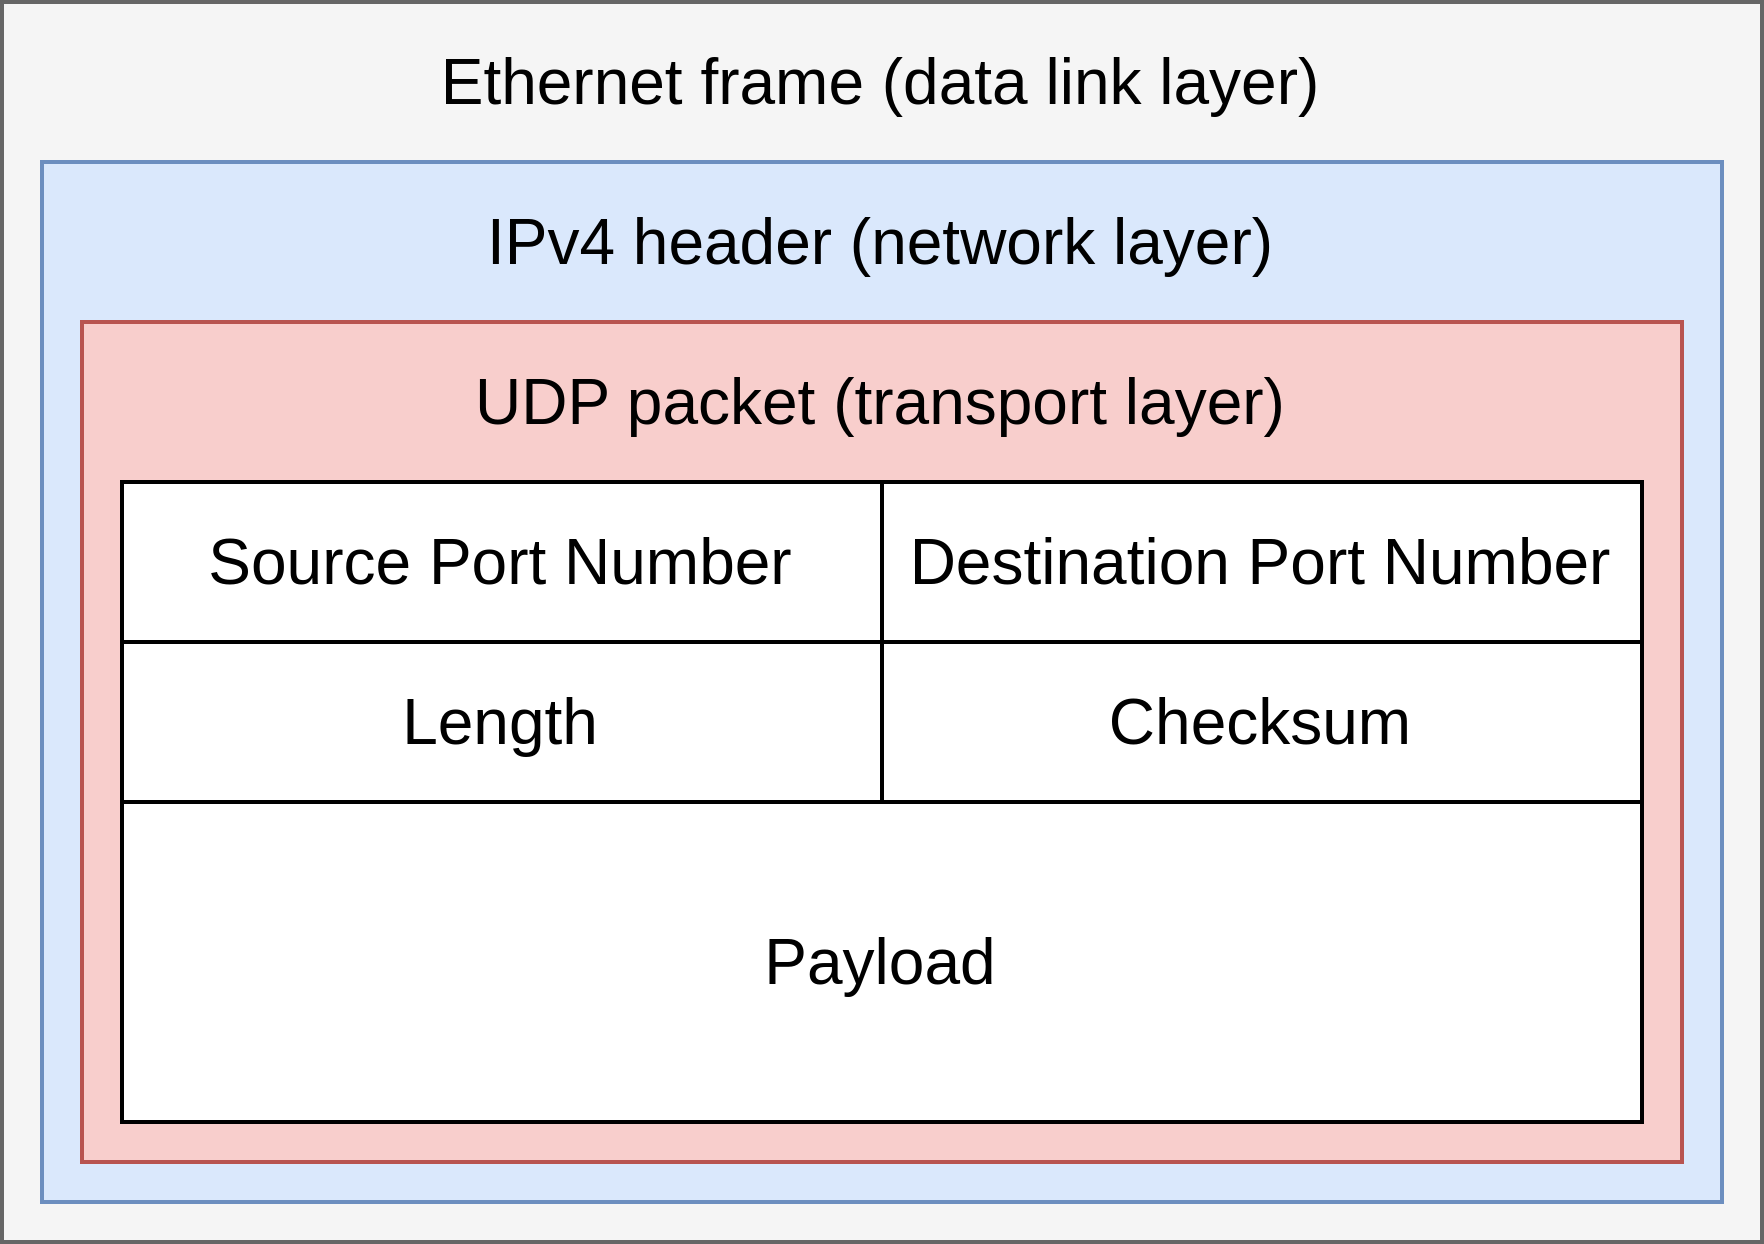
\includegraphics[width=.5\textwidth]{figures/udp}
    \caption{Structure of an ethernet frame containing a UDP packet.}
    \label{fig:udp-frame}
\end{figure}

A UDP packet consists of data encoded in 8-bit integer format.
Being a transport layer protocol, a UDP packet is in fact preceded in an
ethernet frame by information relating to lower layers in the OSI hierarchy: the
network layer and the data link layer.
The structure of a UDP packet (within an ethernet frame) is shown in
\figref{fig:udp-frame}.

\codeinputlisting[float=h]
{text}
{listings/udp-packet.txt}
{Network capture: ethernet frame containing a UDP packet}
{packet-hello-world}
\noindent
The ethernet frame in \lstref{listing:packet-hello-world} was generated
using the Netcat (\texttt{nc}) command line utility\footnote{
    \url{https://nc110.sourceforge.io/}
}, and captured with Wireshark network traffic analysis software.
Four-digit numbers to the left indicate the hexadecimal index of the byte
at the beginning of the corresponding line.
The central block of two-digit hexadecimal numbers are a representation of the
bytes in the ethernet frame, labelled above by byte position.
The block of characters to the right are the same data encoded as ASCII
characters.

\begin{table}[h]
    \centering
    \begin{tabular}[h]{c c c c}
        Start           & End             & Purpose                 & Value                                        \\
        \midrule[1pt]
        \texttt{0x0000} & \texttt{0x000d} & Ethernet header         &                                              \\
        \midrule
        \texttt{0x0000} & \texttt{0x0005} & Destination MAC address &                                              \\
        \texttt{0x0006} & \texttt{0x000b} & Source MAC address      &                                              \\
        \texttt{0x000c} & \texttt{0x000d} & Ethernet frame type     & \texttt{0x0800}: IPv4                        \\
        \midrule[1pt]
        \texttt{0x000e} & \texttt{0x0021} & IPv4 header             &                                              \\
        \midrule
        \texttt{0x0017} & \texttt{0x0017} & Protocol                & \texttt{0x11}: UDP                           \\
        \texttt{0x001a} & \texttt{0x001d} & Source IP address       & \texttt{0xac1efedf}: \texttt{172.30.254.223} \\
        \texttt{0x001e} & \texttt{0x0021} & Destination IP address  & \texttt{0x7f000001}: \texttt{127.0.0.1}      \\
        \midrule[1pt]
        \texttt{0x0022} & \texttt{0x0029} & UDP header              &                                              \\
        \midrule
        \texttt{0x0022} & \texttt{0x0023} & Source port number      & \texttt{0xed3f}: \numDec{60735}              \\
        \texttt{0x0024} & \texttt{0x0025} & Destination port number & \texttt{0x22b8}: \numDec{8888}               \\
        \texttt{0x0026} & \texttt{0x0027} & Length                  & \texttt{0x0016}: \numDec{22}                 \\
        \midrule[1pt]
        \texttt{0x002a} & \texttt{0x0037} & UDP Payload             &                                              \\
        \bottomrule
    \end{tabular}
    \label{tab:packet-structure}
    \caption{Description of selected fields in the UDP packet depicted in
    \lstref{listing:packet-hello-world}.}
\end{table}

Bytes \texttt{0x0000} to \texttt{0x000d} make up the ethernet header,
consisting of the media access control (MAC) addresses of the destination and
source; the final two bytes of the ethernet header, \texttt{0x0800}, indicate
that this is an \textit{internet protocol version 4} frame.
Bytes \texttt{0x000e} to \texttt{0x0021} are the IPv4 header; this contains
information about the internet protocol part of the packet, such as its length
in bytes \textemdash{} \texttt{0x002a} (\numDec{42}) \textemdash{} and
the source and destination IP addresses, encoded as groups of four-bytes.
The source IP address, for example, is \texttt{0xac1efedf}, a 32-bit encoding
of the more familiar-looking \texttt{172.30.254.223}.

Beginning at byte \texttt{0x0022} is the UPD header.
This contains the source port (\texttt{0xed3f}, \numDec{60735}), destination
port (\texttt{0x22b8}, \numDec{8888}), the length of the UDP part of the frame
(\texttt{0x0016}, \numDec{22} bytes) and ends with a checksum, which
can be used to verify the integrity of the packet\footnote{
    In the remainder of this work it is assumed that transmission over LAN is
    unlikely to result in packet corruption; the UDP checksum is not used.
}.
The packet payload begins at byte \texttt{0x002a}, and consists of bytes
corresponding with the ASCII characters \texttt{Hello, world!}, plus
\texttt{0x0a}, the line feed (LF) character, captured and sent by Netcat when
the user hit the return key.

Netcat takes data supplied to a computer's standard input stream, in this
case characters supplied to a terminal emulator, and uses this data as the
payload for the packet to be transmitted.
The payload of a UDP packet can of course consist of any data which can be
appropriately byte-encoded, such as a stream of audio samples, or audio control
data such as MIDI or OSC messages.

Ethernet frames, and UDP datagrams by extension, are subject to size
limitations.
The maximum transmissible unit (MTU) of a transport medium is the limit on the
size of a packet that can be sent without fragmentation, i.e.\ without being
split into multiple sub-packets.
Two bytes (sixteen bits) are allocated to the `Total Length' field of the IPv4
header, which suggests an MTU of $2^{16}-1=~$\num{65535} bytes;
in practice, however, the data link layer imposes a basic limit of \num{1500}
bytes on the payload of an ethernet
frame~\citep{schiavoni_alternatives_2013,ieee_ieee_2018}.

\subsection{Hardware Platforms}\label{subsec:hardware-platforms}

The notion of taking a distributed approach to DSP is reliant on the
identification of a suitable supporting hardware platform.
For an accessible, distributed audio application, the ideal computing platform
should be small and inexpensive, plus easily and rapidly programmable;
of course, it should also provide audio and networking hardware, and, ideally,
well-documented APIs for programming and interacting with this hardware.

Recent years have seen the emergence of a number of small, low-cost platforms
for embedded systems development, perhaps best known amongst these being the
\textit{Arduino} family of microcontroller development boards,\footnote{
    \url{https://arduino.cc/}
}
whose open-source Software Development Kit (SDK), software libraries, and
Integrated Development Environment (IDE) have greatly improved the
accessibility of development on embedded systems~\citep{michon_embedded_2020}.
Though support for audio is limited via Arduino devices, a number of
audio-specific systems, programmable with the Arduino SDK and IDE, and
operable with many Arduino-compatible add-ons (sensors, displays, etc.), have
been produced;
these include various \textit{ESP32} and \textit{STM32} models, and the
\textit{Daisy} and \textit{Teensy} microcontroller ranges.
These platforms benefit from the wealth of tools, documentation and support
associated with Arduino and the surrounding D.I.Y.\ and maker communities.
Also worthy of consideration are the \textit{Raspberry Pi} and \textit{Bela}
platforms.
Though these are \textit{Embedded Linux Systems} rather than microcontrollers,
%\textemdash{} Bela is an audio ``cape'' for the \textit{BeagleBone Black}
%single-board computer, and a variety of audio breakout-boards exist for
%producing high quality audio output with Raspberry Pi models \textemdash{}
they are small-footprint devices, suitable for embedded applications.
Bela in particular has been designed with a focus on audio development and
interaction via sensors; it can be programmed via an accessible, web-based IDE,
and the user need not interact with the underlying Linux operating system.
Raspberry Pi is less approachable for audio development, and tends to be
operated as more of a general-purpose small computer, though support for
treating the platform like a microcontroller \textemdash{} taking a
\textit{bare metal} approach \textemdash{} is offered via the \textit{Circle}
environment.\footnote{\url{https://github.com/rsta2/circle}}

The above systems are typically programmed in C++, with support for audio
development provided by libraries such as Daisy's \textit{DaisySP} and Teensy's
\textit{Teensy Audio Library}, which each provide audio APIs and a selection of
pre-made algorithms for audio synthesis and DSP.\
Bela, as an alternative to its C++ audio API, can be programmed with the
graphical programming language PureData, and Teensy, as a complement to its
Audio Library, offers a web-based \textit{Audio System Design Tool}, via which
the user may describe an audio system diagrammatically and export the result to
C++.

This profusion of approaches, and a variety of platform-specific APIs, can
render embedded audio development somewhat difficult to approach.
A concerted effort has been made, however, by the community behind the
\textit{Faust} programming language,\footnote{\url{https://faust.grame.fr/}} to
provide support for embedded platforms.
Faust is a functional paradigm, audio domain-specific language, that was created
to serve as a ``viable and efficient alternative to
C/C++''~\citep{orlarey_faust_2009} for the development of audio applications on
a variety of platforms.
In Faust, a user can write high level sound synthesis or DSP code and export the
result to C++ that meets the requirements of the audio API on a given target
platform.
This is achieved via a series of platform-specific ``architecture files'' and
Faust's \texttt{faust2[...]} tools,\footnote{
    \url{https://faustdoc.grame.fr/manual/tools/}
} which include
\texttt{faust2bela}, \texttt{faust2teensy}, etc.~\citep{michon_real_2019,
    michon_embedded_2020}.
Developers are thus able to focus on writing audio code, rather than being
concerned with the peculiarities of the device or system upon which they wish
to deploy their program;
further, Faust's support for a variety of embedded platforms facilitates testing
and rapid prototyping.

\begin{table}[t]
    \centering
    \begin{tabular}{ c c c r }
        Platform &
        Processor &
        Memory &
        Price \\

        \midrule

        Teensy 4.1\tablefootnote{\url{https://pjrc.com/store/teensy41.html}} &
        ARM Cortex-M7 \qty{600}{\MHz} &
        \qty{1}{\mega\byte} SDRAM &
        \texteuro{32} \\

        Daisy Seed\tablefootnote{\url{https://electro-smith.com/daisy/daisy}} &
        ARM Cortex-M7 \qty{480}{\MHz} &
        \qty{64}{\mega\byte} SDRAM &
        \texteuro{28} \\

        ESP32-LyraTD\tablefootnote{\url{https://espressif.com/en/products/devkits/esp-audio-devkits}} &
        Dual core Xtensa LX6 \qty{240}{\MHz} &
        \qty{8}{\mega\byte} PSRAM &
        \texteuro{19} \\

        STM32H747I\tablefootnote{\url{https://st.com/en/evaluation-tools/stm32h747i-disco.html}} &
        ARM Cortex-M7 \qty{480}{\MHz} + M4 \qty{240}{\MHz} &
        \qty{1}{\mega\byte} RAM &
        \texteuro{94} \\

        Bela\tablefootnote{\url{https://shop.bela.io/products/bela-starter-kit}} &
        ARM Cortex-A8 \qty{1}{\GHz}\tablefootnote{\url{https://beagleboard.org/black}} &
        \qty{512}{\mega\byte} SDRAM &
        \texteuro{190} \\

        Raspberry Pi 4\tablefootnote{\url{https://www.raspberrypi.com/products/raspberry-pi-4-model-b/}} &
        ARM Cortex-A72 \qty{1.8}{\GHz} &
        \qtyrange{1}{8}{\giga\byte} SDRAM &
        \texteuro{30-100}
    \end{tabular}
    \caption{Comparison of selected embedded audio development platforms.
    Prices as of January 2024.}
    \label{tab:embedded-comparison}
\end{table}

A comparison of selected devices can be found in
\tabref{tab:embedded-comparison}.
Bela is significantly more powerful than the microcontroller systems, but it is
commensurately costly.
The Raspberry Pi is also very capable, and a model with \qty{1}{\giga\byte} RAM
may cost as little as \texteuro{30};
its operating system stands as an impediment, however, to implementations that
seek to prioritise audio functionality above all.
Support for bare metal development on Raspberry Pi is not comprehensive, and
there is no Faust tool to produce code that is compatible with Circle.
Daisy Seed is well-appointed with memory (which is important for DSP algorithms
featuring long delay-lines, for example), but does not feature ethernet support.
Teensy 4.1, and the selected ESP32 and STM32 devices support networking via
ethernet add-ons, but the ESP32's CPU is underpowered, and the STM32 is
unfavourably-priced.
Though lacking in memory, Teensy's processor, low price, and networking support
make it an attractive candidate platform for a distributed, networked audio
implementation.
Further, thanks to the presence of a vibrant developer community, utilities such
as \textit{TyTools}\footnote{\url{https://koromix.dev/tytools}} exist, and can
be used to program multiple Teensy devices in a single command \textemdash{}
useful for a system distributed amongst many such devices.

One respect in which Teensy is found wanting is audio fidelity.
By default, its audio add-on (or \textt{shield}) produces CD quality output
(16-bit, \qty{44.1}{\kHz}), falling short of modern requirements for
high-quality audio, such as offered by Daisy Seed (24-bit, \qty{96}{\kHz}).
While Teensy's sampling rate can be increased, sample resolution is fixed by
the Teensy Audio Library and at the level of the audio codec.
In spite of this shortcoming, and in light of its other, more advantageous
qualities, Teensy was selected as the platform upon which to conduct
development.

\subsection{Audio Spatialisation}\label{subsec:audio-spatialisation}

Audio spatialisation is, plainly put, the practice of distributing sound in
space.
In terms of the reproduction of \textit{primary sound sources}, i.e.\ sound
captured by microphones, recorded as digital audio files, or synthesised in
real-time, spatialisation can be achieved simply by delivering those primary
sources to \textit{secondary sound sources}, i.e.\ loudspeakers, placed at
arbitrary positions relative to a listener.
Such an approach is, of course, inflexible;
loudspeakers being stationary entities by-and-large, the idea of moving a sound
source is physically impractical, and, that of locating a sound source
between loudspeaker positions physically impossible.
Taking advantage of auditory cues, however, and the nature of the propagation
of sound, it is possible to suggest the presence of primary sources at
arbitrary locations, independent of the secondary source distribution.
The motivation behind audio spatialisation, then, is to create (or indeed
\textit{recreate}) sonic environments for creative and immersive purposes, such
as for virtual reality experiences, in cinematic settings, for music production
or art installations, to give but a handful of examples.

A number of techniques exist for what is termed \textit{sound field
synthesis}~\citep{ahrens_analytic_2012,nicol_sound_2017}, all of which
essentially take the form of applying some manner of \textit{driving function}
to an input audio signal to generate an appropriate driving signal to be
delivered to a secondary sound source in the listening
environment~\citep{ahrens_analytic_2012}.
For a loudspeaker at position $\mathbf{x} = \begin{bmatrix}
                                                x & y & z
\end{bmatrix}^T$, the driving signal $\hat{D}(\mathbf{x}, \omega)$ can be
expressed, in the frequency domain, as the product of the input signal,
$\Sigin(\omega)$ and the driving function $D(\mathbf{x}, \omega)$:
\begin{equation}
    \label{eq:driving-signal-freq}
    \hat{D}(\mathbf{x},\omega) = \Sigin(\omega) \cdot D(\mathbf{x},\omega),
\end{equation}
where $\omega$ denotes radian frequency, $\omega = 2\pi f$, and $f$, in turn,
is time frequency.
Moving to the time domain, the multiplication of the input signal and driving
function changes to a convolution, and equation~\eqref{eq:driving-signal-freq}
becomes:
\begin{equation}
    \label{eq:driving-signal-time}
    \hat{d}(\mathbf{x},t) = \sigin(t) \ast d(\mathbf{x},t),
\end{equation}
where $t$ denotes time.

An early sound field synthesis approach, referred to as an `acoustic
curtain'~\citep{ziemer_wave_2020} entailed placing microphones in one space,
such as a concert auditorium, and, in another space, loudspeakers at locations
corresponding to those of the microphones.
In this case, there are as many input signals $\hat{S}_k(\omega)$ as there are
microphones, and the driving function reduces to a `pass-through' of each
signal to its corresponding loudspeaker, i.e. $D_k(\mathbf{x}, \omega) = 1$.

The acoustic curtain is a relatively rarely-deployed technique (though similar
recreation of `real' sound fields is still conducted, albeit typically by way
of ambisonic recording and reproduction) and sound field synthesis is most
often concerned with the distribution and movement of artificial or arbitrary
sound sources.
Commonly-employed approaches to sound field creation can be grouped into two
broad categories: amplitude- and time-based panning techniques, and physical
sound field recreation approaches.

\subsection{Periphony}\label{subsec:periphony}

The former, \textit{periphonic}, types are perhaps more familiar to the
layperson and encompass stereophony and surround-sound systems, consisting of
secondary sources in a horizontal planar arrangement equidistant to the
listening position.
These techniques exploit the interaural level difference (ILD) cue, i.e.\ the
difference in perceived amplitude relative to the listener's
ears~\citep{pulkki_virtual_1997,verheijen_sound_1998,ziemer_wave_2020}, to
encourage the listener to localise sound to a position on the circumference of
an arc or circle around the listening position.
This is achieved by weighting the amplitudes of signals sent to the
secondary sources, creating a ``phantom'' sound source that may appear to
emanate from a position between loudspeakers.
For systems of this sort, the driving function is a constant scalar value, or,
for a moving phantom source, a time-varying function that returns a scalar
value.
Such periphonic approaches can extend to three dimensions in the case of
vector base amplitude panning (VBAP)~\citep{pulkki_virtual_1997}, which uses
trios of speakers to position phantom sources on the surface of a sphere
with the listening position at its origin.

Time-based panning effects, by contrast, make use of the interaural time
difference (ITD) cue to give the impression of a phantom source located toward
the loudspeaker producing the signal at the earliest
time~\citep{pulkki_virtual_1997,verheijen_sound_1998}.
Thus the driving function for a time-based panning system is a delay of the
form:
\begin{equation}
    d(\mathbf{x},t) = \delta(t - \tau),
    \label{eq:time-driving-function}
\end{equation}
where $\tau$ is the duration of the delay.

The effects of ILD and ITD cues may transfer to headphone-based listening,
in which case, rather than periphonic, they become a sort of \textit{in-head}
localisation~\citep{ahrens_analytic_2012}.
It is worth mentioning that these cues vary in their effectiveness with
frequency and, excepting the case of headphone-based listening, intersect with
cues related to listener's torso~\citep{verheijen_sound_1998} and the
head-related transfer
function~\citep{de_poli_physically_1998,geier_object-based_2010}.

Periphonic approaches (again, headphones excepted) are subject to the
phenomenon of an ideal listening position, or
\textit{sweet-spot}~\citep{verheijen_sound_1998,nicol_sound_2017}, that is a
listening position away from which the spatialisation effect is significantly
degraded.
As such, these techniques are not suited to subjection to multiple listeners,
nor to immersive auditory experiences permitting the participant to move freely
about their environment.
Additionally, phantom sources are inherently bound to the periphery on which
they reside;
there is no authentic way to model a phantom source at greater (or lesser)
distance, though using reverberation and amplitude cues may offer a satisfactory
perceptual impression.

\subsection{Physically-Inspired Techniques}

\begin{figure}[ht]
    \centering
    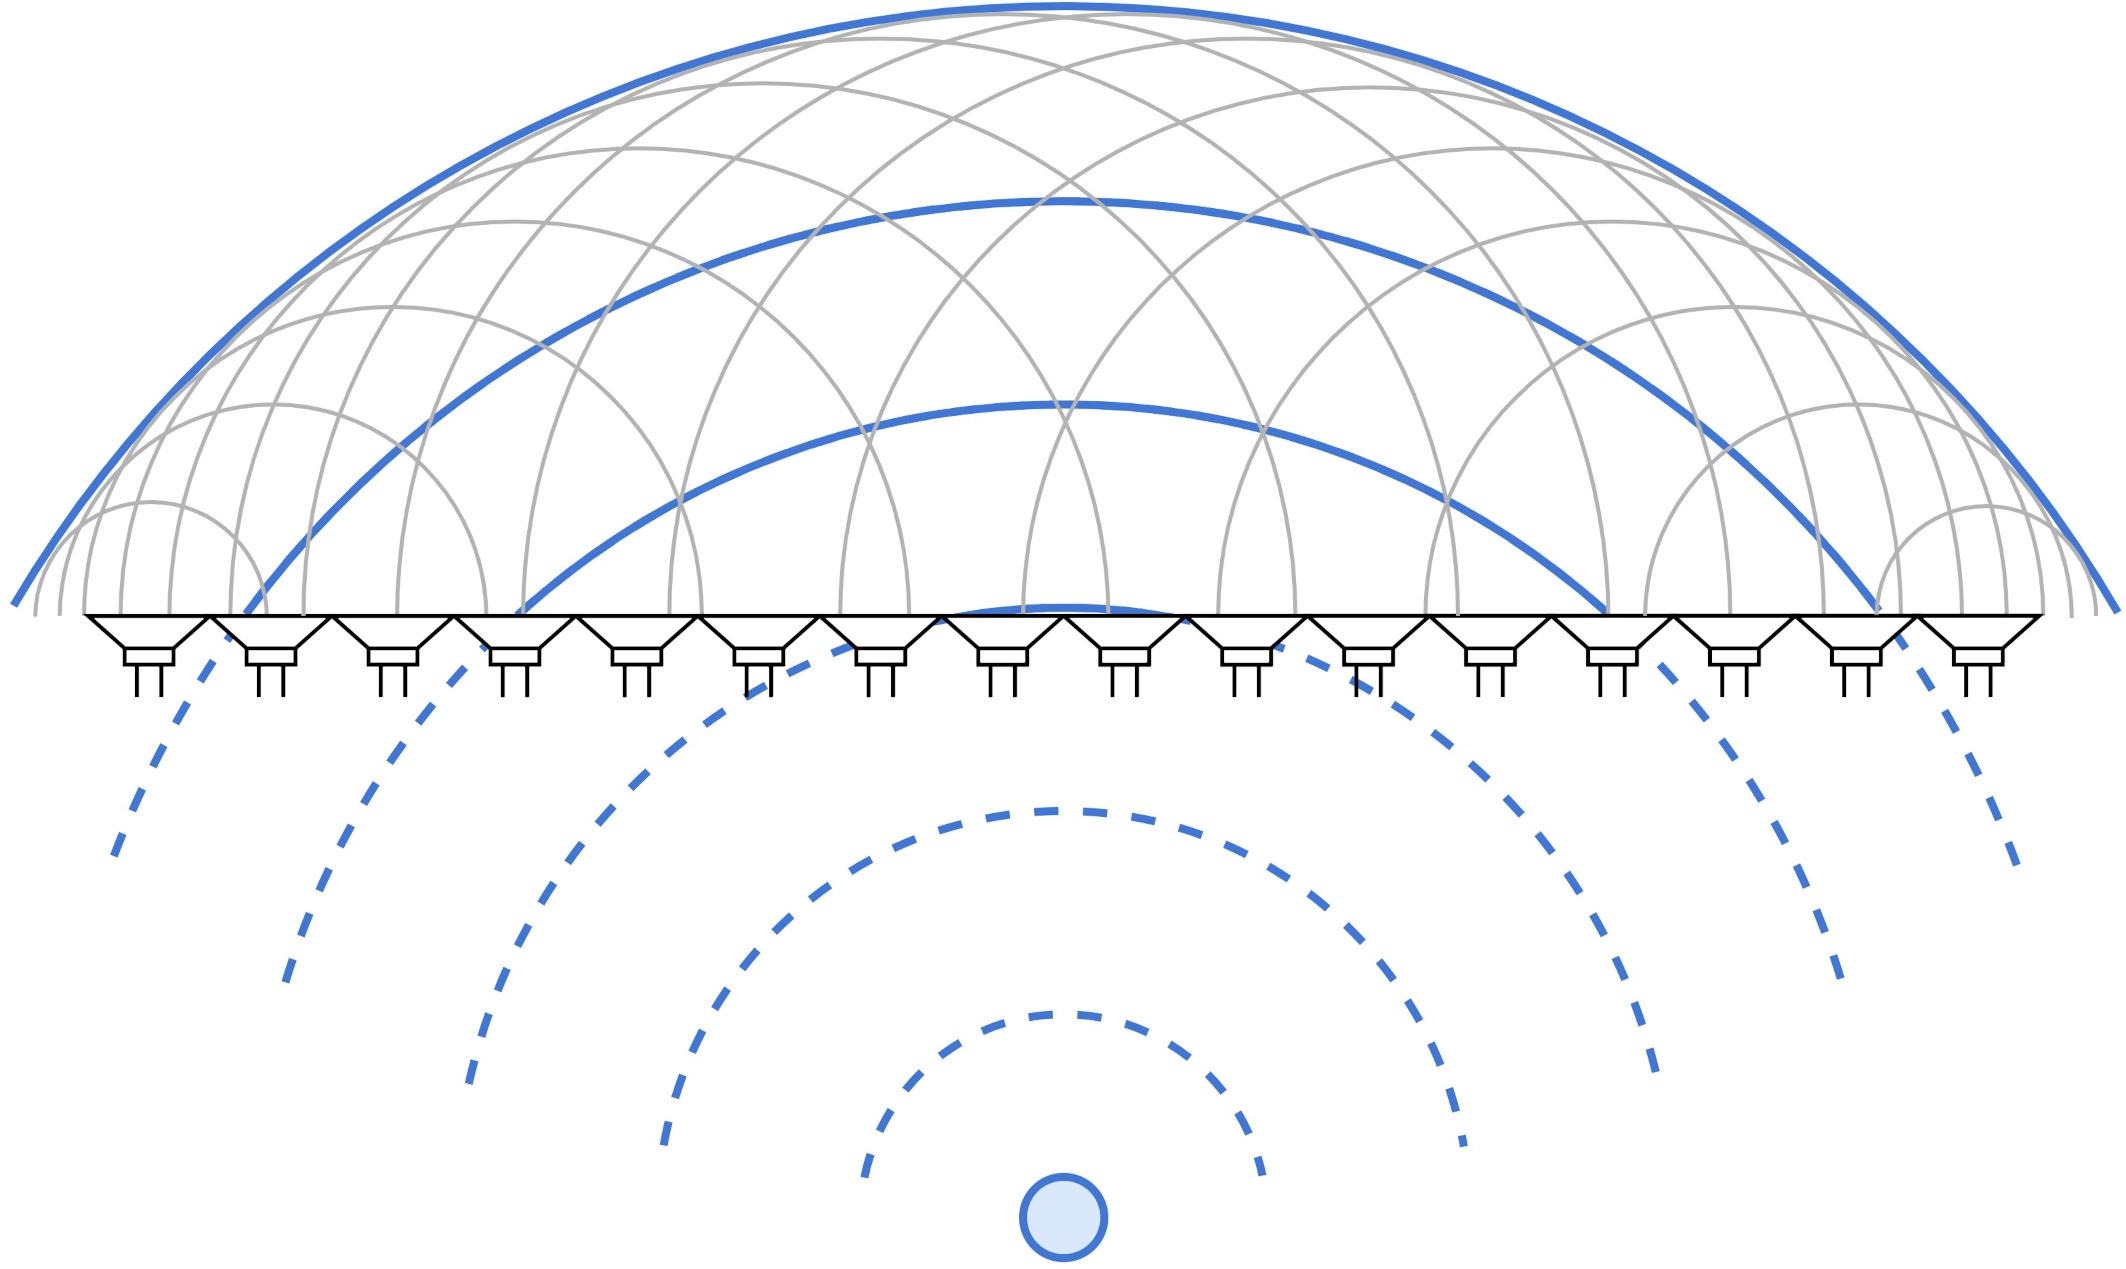
\includegraphics[width=\textwidth]{figures/wfs_1}
    \caption{\textit{Holophony}.
    Huygens' principle states that the propagation of a wavefront
    can be recreated by a collection of secondary point sources.
    The bottom of the figure represents a virtual sound field, and the top a
    real sound field, separated by a row of secondary point sources
        (loudspeakers).
        The small blue circle represents a virtual sound source and the blue
        dashed arcs are virtual wavefronts associated with that sound source;
        the grey arcs are wavefronts produced by the array of secondary point
        sources;
        the solid blue arcs represent the propagation of a reconstructed
        wavefront in the real sound field.}
    \label{fig:wfs_1}
\end{figure}

Physical approaches fall into two main types: wave field synthesis (WFS) and
ambisonics (and higher-order ambisonics \textemdash{} HOA). Rather than
directly manipulating sound localisation cues, these types seek to trigger
those cues indirectly by synthesising a sound field as if it had been created
by `true' acoustic sources, as opposed to loudspeakers.
In the case of ambisonics, the sound field is decomposed into `spherical
harmonics', spatial functions described by linear sums of directional
components of increasing order~\citep{nicol_sound_2017}.
Spherical and plane waves can be reproduced, corresponding with virtual
point sources and sources at `infinite distance' respectively.

Ambisonics, like periphonic approaches, suffers from a sweet-spot effect which
worsens with attempts to reproduce sounds of higher frequency.
The ideal listening area can be broadened by implementing ambisonics at higher
order, increasing the density of the distribution of secondary sources.
Doing so obviously has ramifications for the physical complexity of an
ambisonics installation, and, since higher-order spherical modes must be
calculated, in terms of computational demands placed on the system.

\subsubsection{Wave Field Synthesis}

Reminiscent of the acoustic curtain, WFS is based upon Huygens' principle,
originating in the field of optics, which states that a propagating
wavefront can be recreated by a distribution of secondary point
sources~\citep{mueller_acoustic_1971,berkhout_acoustic_1993,
    belloch_performance_2021}(see \figref{fig:wfs_1}).
It is variously termed a form of \textit{acoustic holography} or
\textit{holophony}~\citep{berkhout_holographic_1988,ahrens_analytic_2012}.
Effectively, by timing the reproduction of an input signal at an array of
secondary sources, a wavefront associated with a virtual sound source can be
synthesised.
To simulate distance cues, a filter can be applied to model losses to the
virtual medium of acoustic propagation.
The principle assumes a continuous array of secondary sources but of course in
practice it is necessary to use a discrete array of loudspeakers, which,
much as is the case with HOA, has ramifications for spatial resolution;
to mitigate the issue of spatial aliasing, whereby sounds of higher frequency
cannot be recreated unambiguously~\citep{winter_geometric_2018},
secondary sources should be placed very close together.
Consequently, to serve a large listening area, many speakers, and thus many
audio channels, are required.

Via appropriate timing of the delivery of a primary sound source to the
secondary source array, it is possible to synthesise virtual sound sources,
plane waves, and \textit{focused} sound sources, corresponding with concave,
flat, and convex synthesised wavefronts respectively; the latter, dependent
on the location of the listener, appear to emanate from within the real
sound field, rather than its virtual counterpart.

\begin{figure}[ht]
    \centering
    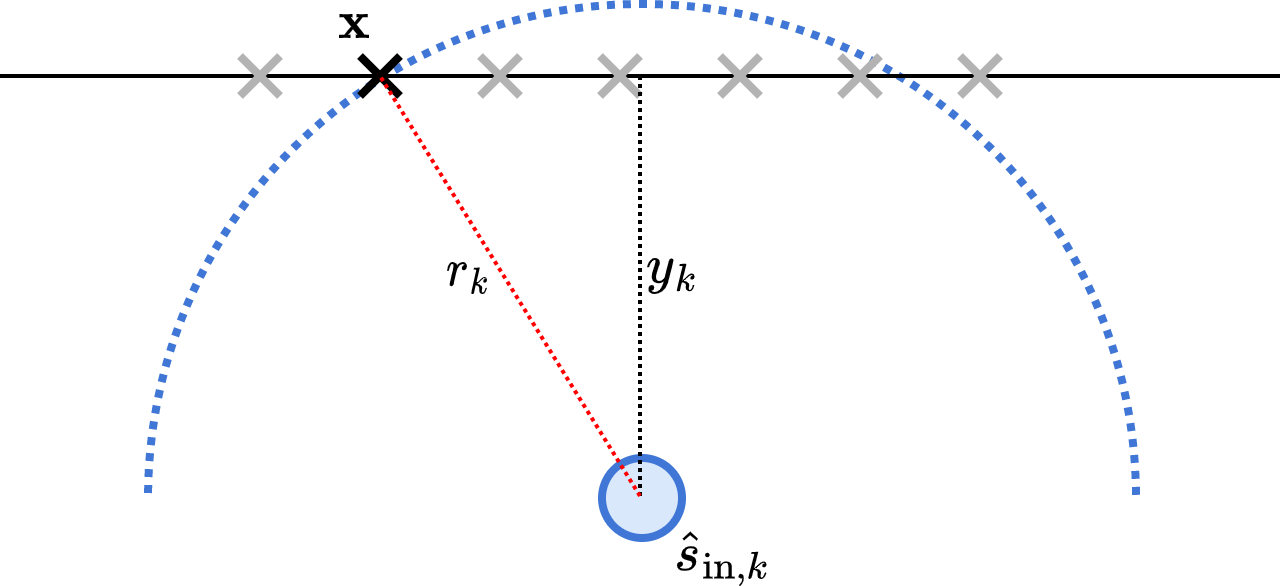
\includegraphics[width=.75\textwidth]{figures/wfs_2}
    \caption{
        The driving signal for the WFS secondary source at position $\bfx$,
        for virtual primary source $\sigink$, is dependent on the distance
        $r_k$ of the primary source from the secondary source.
        This corresponds with a propagation delay via the simulated medium of
        propagation, coupled with a filter describing losses to that medium.
    }
    \label{fig:wfs_2}
\end{figure}

Focusing on the former kind, however, for $m$ virtual sources, the time-domain
driving signal $\hat{d}$ for the secondary source at $\bfx$ may be expressed
as:
\begin{equation}
    \hat{d}(\bfx,t) = \sum_{k=0}^{m-1}\sigink \ast d_k(\bfx,t),
\end{equation}
where the driving function $d_k$ is~\citep{ahrens_analytic_2012}:
\begin{equation}
    \label{eq:driving-function}
    d_k(\bfx,t) = \frac{y_k}{r_k}f(t) \ast \delta\left(t - \frac{r_k}{c}\right).
\end{equation}
The \textit{WFS prefilter}~\citep{ahrens_analytic_2012} $f(t)$ is a function that
aims to simulate the absorption of energy into the simulated medium
of acoustic propagation.
The delta function $\delta$ has the effect of delaying the prefilter, and thus
$\sigink$, by the time of propagation for a medium with propagation speed $c$
(typically modelled as \qty[per-mode=symbol]{343}{\m\per\s} for sound in air).
The components of the driving function are depicted in \figref{fig:wfs_2}.

\subsection{Distributed Computing}\label{subsec:distributed-computing}

In the broadest terms, a distributed system is \textit{``a collection of
independent entities that cooperate to solve a problem that cannot be
individually solved''}~\citep{kshemkalyani_distributed_2011}.
In turn, the term \textit{distributed computing} simply describes a system of
computation that is distributed in
space~\citep{lamport_distributed_1990}.\footnote{
    There is a certain linguistic symmetry here with respect to spatial audio,
    but that is as far as the parallel goes.
}
At a low enough level, this effectively describes \textit{any} computer
system, such systems being composed of individual entities \textemdash{}
processors, memory, input and output devices, etc. \textemdash{} all
acting in cooperation.

At a higher level \textemdash{} that of a computer network, for example
\textemdash{} why take a distributed approach to computation?
As Kshemkalyani and Singhal describe~\citep{kshemkalyani_distributed_2011},
a variety of rationales exist for taking such an approach;
adapting these to the notion of distributing an audio spatialisation algorithm
across a computer network, most relevant are:

\textbf{Scalability}
Particularly so if taking advantage of a network protocol that supports
multicast or broadcast transmission.
Under a unicast model, such as that employed by JackTrip, streams of audio data
are duplicated on a per-client basis;
under such a model, at some point all available network bandwidth will be
exhausted.
An ideal multicast networked audio system entails there being just one stream
of audio data, plus perhaps a stream of control data, for all clients to
consume.
Dependent on the application, the server in such a system may not need to be
aware of how many clients are connected; similarly, clients exist in isolation,
and fulfil their task with no dependency on their peers on the network.

\textbf{Modularity}
Closely related to scalability, modularity entails \textit{extensibility}.
This is something that centralised audio spatialisation systems either lack
entirely, or possess only at great cost in terms of hardware, and even then only
if the hardware supports extension via daisy-chaining, for example.
%The matter of expense anticipates:\textemdash{}

\textbf{Improved cost/performance ratio}
A modular, scalable system can be constructed to meet the proportion that
circumstances require, with the minimum amount of redundancy.
If it becomes desirable to scale the system up, this can be achieved by small
increments rather than by expensive leaps.\\

Kshemkalyani and Singhal also vaunt \textit{enhanced reliability} as motivation
for distributed computing.
This may indeed hold true for systems where the failure of a single node can be
compensated for by increased work on the part of the remaining nodes until such
time as the failed node can resume operation or be replaced;
it does not for the sort of system under consideration here.
Indeed, this points toward two significant drawbacks of distributed systems in
general: increased complexity and a proliferation of potential points of
failure.
Nodes in a distributed computational system must be served at the very least
with power and access (e.g.\ over a network) to the data that they require in
order to operate.
This entails the provision of cables, perhaps batteries, and physical
connections that may be subject to wear-and-tear or misuse.
Additional concerns surround the programmability of such a system, which is the
other side to the coin of modularity;
integrity, in terms of all nodes possessing up-to-date instructions for
operation, may be difficult to ensure.

\subsection{Distributed Audio Systems}\label{subsec:distributed-audio-systems}

The notion of taking a distributed approach to audio processing is by no means
unprecedented;
a selection of prior work in distributed DSP and audio spatialisation, plus
systems incorporating microcontrollers and single-board computers is detailed
below.

\subsubsection{State of the Art}

Applications of SoundWIRE to what its creators termed \textit{Internet
Acoustics}~\citep{chafe_physical_2002} obviously represent a case of distributed
audio processing.
These include implementations such as a network
reverberator~\citep{chafe_i_2018}, or
\textit{``transcontinental echo chamber''}~\citep{chafe_simplified_2000},
plus the aforementioned \textit{Network Harp}.
Experiments of this sort were intended initially as sonifications of QoS
\textemdash{} a characteristic of network systems that is difficult to represent
in graphical or textual form due to the ephemeral nature of phenomena such as
jitter and packet loss \textemdash{} but stand as fascinating applications in
their own right of digital audio in the age of computer networking.
Subsequent work on JackTrip has focused on optimising networked audio less
for sound processing or as a creative tool in itself, and more in service of
the social and communal aspects of music participation and appreciation in a
networked world;
these are topics that came to the fore in computer music research during the
COVID 19 pandemic~\citep{bosi_experiencing_2021,sacchetto_jacktrip-webrtc_2021}.

Lago~\citep{lago_distributed_2004} proposed a UDP-based system for real-time
distributed audio processing taking the form of a network of general purpose
computers.
A server sent packets of audio data to be processed by a collection of
clients, which would then return processed audio to the server to be combined
and used for output.
Since clients were not to be used directly for output, synchronisation was not
important, but Lago identifies the timing or hardware based interrupts for
audio and network processing as being of great importance to a distributed
real-time implementation.
Though an interesting exploration of approaching certain difficulties of
distributed computing, DSP in particular, and ambitious for its time (2004),
arguably the need for such a system has been obviated by advances in computer
processing power over the succeeding two decades.

A digital music production system of networked Beagleboard single-board
computers was demonstrated by Gabrielli et al.~\citep{gabrielli_networked_2012}
Another ambitious project, particularly since it relied on wireless
communication, the authors describe an interesting way of measuring
transmission round-trip times.\todo[inline]{See section about test signals?}

Exploring the possibilities of burgeoning network technology in the early 2010s,
Lopez-Lezcano set out to build a UDP-based `network sound card' to support
a networked WFS system~\citep{lopez-lezcano_jack_2012}.
The aim was to replace otherwise expensive high channel-count conventional
audio interfaces, which receive audio over the MADI (Multichannel Audio Digital
Interface) protocol, with a more cost-effective alternative.
Ultimately the devised system was not used for audio spatialisation, but
facilitated networked musical performance, and it stands as an example of the
results that can be achieved by using `raw' UDP data for audio transmission,
rather than an established protocol or system.

In addition to Gabrielli et al., implementations on IoT-like devices include
Chafe and Oshiro's port of JackTrip to the Raspberry Pi single-board computer
for further internet acoustics, plus distributed spatialisation systems such as
those described by Devonport and Foss~\citep{devonport_distribution_2019} and
Belloch et al.~\citep{belloch_performance_2021}
The latter two address aims closely aligned with the work described here, but
are based on costly computing platforms.
Devonport and Foss achieved high synchronicity via AVB; Belloch et al. used a
GPU-based hardware platform, which is perhaps unsuited to its task, and report
client synchronisation to the millisecond range \textemdash{} likely not
sufficient for timing-critical audio spatialisation effects.

Also of interest is the OTTOsonics~\citep{mitterhuber_ottosonics_nodate}
project;
its emphasis on a fully-costed, do-it-yourself alternative to conventional
spatial audio systems is pertinent to this work, though it diverges in its use
of AVB, and associated hardware for audio transmission.

\subsection{Challenges}\label{subsec:challenges}

Time, especially when dealing with the fine margins posed by real-time audio
processing, represents the principal source of difficulty in a distributed
audio setting.

\textit{Jitter} refers to fluctuations in the rate of transmission or
processing.
In a networked audio setting, jitter gives rise to a situation whereby the
arrival of audio data does not correspond with the moments at which it is
needed.
In a naive implementation, this may result in a recipient either halting
processing until it receives the expected data, or simply continuing without
any data.
In either case, the result is likely to be disruption of the integrity of the
audio signal in the form of audible discontinuities.

\textit{Clock drift} arises as an inevitable consequence of no source of time
in a system of computation being perfectly uniform, and no two sources of time
being identical.
The timing of a computer system is typically governed by a crystal oscillator,
the accuracy of which is affected by factors such as ambient temperature, and
potentially computational load on the system it
governs~\citep{marouani_internal_2008}.
Relative drift (sometimes, within the diagnostic parts of JackTrip for example,
referred to as \textit{skew}), is the difference in clock rates between two or
more systems.
Whereas jitter is a short-term phenomenon, clock drift typically takes effect
over a longer timescale.
As two distinct systems of time move in and out of phase with each other over
the longer term, drift may indeed give rise to jitter.

In studio and professional audio settings, devices may be synchronised via an
authoritative clock source such as word clock, or, in a networked setting,
via PTP or lower-resolution network time protocol.
In the absence of such an authoritative source, e.g.\ over a wide area network,
or if using hardware that does not support such measures, buffering strategies
are typically employed, coupled with delay-locked
loops~\citep{adriaensen_using_2005} and
resampling~\citep{adriaensen_controlling_2012}.


\section{Research Questions}\label{s:research-questions}

The primary focus of this thesis is an exploration of employing a
network of hardware modules to act as a co-ordinated networked-audio system
with a view to supporting a distributed approach to audio spatialisation
techniques.
It is hoped that in selecting a low-cost hardware platform, using ubiquitous
computer networking technologies, and keeping the overall design as simple as
possible, the work here could lead to a lowering of the barrier to entry of
the creation of large scale spatial and immersive audio installations.
The first research question, then, is:

\begin{researchq}
    \label{rq:rq1}
    How can a network of microcontrollers be used to create a distributed
    audio system suitable for managing scalable installations for spatial
    and immersive audio?
\end{researchq}

\noindent
Adjacent to the bare bones of implementation is the performance of the devised
system:

\begin{researchq}
    \label{rq:rq2}
    How can such a system be created and configured such that it maintains
    inter-client synchronicity? What are the effects of loss of
    synchronicity on distributed spatialisation algorithms?
\end{researchq}

% \noindent
% These questions will be our guides in the chapters to follow.

\subsection{Prior Work}

Before beginning work on this project, a distributed WFS system was
developed, based on the Teensy 4.1 microcontroller and JackTrip protocol.
This consisted of an audio application running on a general purpose computer,
delivering audio over JackTrip to a collection of hardware modules, and
WFS control data over multicast UDP.
Strategies were developed for mitigating the effects of jitter and clock drift,
and these serve as the basis for work on the project described in this thesis.

The prior system was not formally evaluated, but, anecdotally, provided
support for the holophonic effect of primary-source WFS.
These strategies were initial efforts, based on a limited understanding
of the problem-space, and called for further development.
It was deemed, also, that the implementation was constrained by the more
opinionated aspects of the JackTrip system.

A paper documenting the work on the JackTrip-based approach can be found in
appendix \ref{ap:jacktrip-teensy}.
